% Chapter 4

\chapter{Technical Analysis} % Main chapter title
 
\label{Chapter4} % For referencing the chapter elsewhere, use \ref{Chapter5} 

\lhead{Chapter 4. \emph{Technical Analysis}} % This is for the header on each page - perhaps a shortened title

%---------------------------------------------------------------------------------------
\section{Introduction}
This chapter investigates whether technical analysis can provide a positive expectancy for financial traders \citep{Kuang2014192, Hsu2010471}. A variety of technical analysis indicators are employed including MACD, Aroon, Stochastics Oscillator and Rate of Change (ROC) indicator. The experimental results from using these indicators are presented in groupings based on the general category of indicator such as trend identification, market reversal and momentum indicators \citep{Taylor2014286}. Some technical indicators have a role to play in more than one area, for example MACD can be considered a trend detection indicator or a market reversal indicator.

The effectiveness of a particular indicator or system is measured in terms of \textquotedblleft points" gained, which is also referred to as \textquotedblleft PL" (which stands for to profit and loss). The results presented in this chapter are mainly based around systems in which a trade is opened and closed each day, producing a daily PL either positive or negative. The sum of all the individual days produces the total system PL and these values are reported in the results tables. For example, if the market moved from 6000 to 6200 in any one day a PL of either 200 (6200 - 6000) or -200 (6000 - 6200) depending upon which way the trade was placed, would be added to the overall system results. 

In addition, the results are presented such that returns from \textquotedblleft going long" (expecting the market to rise) are presented separately from the opposite scenario of \textquotedblleft going short". This is because  market behaviour is often different while it is rising than it is while falling and systems may be more adept at predicting price movements in one of the directions. Further, transactions costs are not taken into account in the results and these would typically be 1 point per trade for the European markets, 2 points for the Dow and 10 for the Nikkei.  Thus if a system made a PL of 1000 but it required 2000 trades at 2 points per trade, in reality the system would have lost money. 

The results presented in this chapter and the following one are based around trading systems. Essentially the methodology concerned, technical analysis in this chapter and time series analysis in the next, attempt to predict future market direction. The values from the various indicators and forecast techniques are fed into a variety of trading algorithms which use the forecast information to decide whether to make long (expect the market to rise) or short (expect the market to fall) trades. For consistency the algorithms all return the same data object containing the following results:

\begin{enumerate}
\item Mkt - the name of the financial market such as DAX, FTSE etc.
\item S Loss - the value of any stop loss applied
\item LongPL - the profit or loss generated from just the \textquotedblleft Long" trades.
\item ShortPL - the profit or loss generated from just the \textquotedblleft Short" trades.
\item L Win \% - the percentage of time the Long trades win.
\item L Trades - the number of Long trades executed.
\item Av L PL - the average profit or loss generated from each Long trade.
\item S Win \% - the percentage of time the Short trades win.
\item S Trades - the number of Short trades executed.
\item Av S PL - the average profit or loss generated from each Short trade.
\item misc - miscellaneous information such as the SMA used in the algorithm.
\end{enumerate}

The results from Long and Short trades in particular trading algorithm are considered separately as frequently markets behave differently as they move up as opposed to as they fall. Further, the percentage of times the algorithm results in winning trades, the number of trades and the average profit or loss (PL) for each trade is reported for both Long and Short trades. The average PL is primarily reported in the following results tables because this allows comparisons between systems that generate a lot of trades with those such as the algorithms based on candlestick patterns that results in only a small number of trades. 

% --------------------------------------------------------------------------------------
\section{Baseline Systems - Naive Methods}
Initially two very simple ideas were explored in order for the results to be used as baselines against which the technical indicators explored in the rest of the chapter and the time series models of Chapter \ref{Chapter5} can be compared. There is an expectation that the use of technical indicators will produce systems that provide much better results than these two so-called naive systems.

The first system simply uses the idea that markets tend to increase in value over time. The algorithm applies a naive approach and simply enters a trade each day expecting the market to rise. The well-known method of "Buy and Hold" applies the same principles. The total PL of the resulting system is the the sum of all the daily close minus open prices. This approach has been named a \textquotedblleft Naive Long System".

The second approach is equally simplistic, and again is based around opening and closing a trade each day. A notable difference from the first naive system is that the algorithm can result in either a buy or a sell (expecting the market to decline in value) occurring. If a market increased in price the previous day the algorithm \textquotedblleft reverses" it and expects the market to fall today. Likewise if the market had fallen the previous day the system buys the market today. This idea has been named the \textquotedblleft Naive Reversing System".

%-----------------------------------------------------------------
% ---------------------------  Naive Long ------------------------
\subsection{Naive Long System}
The results of the naive long system can be seen in Table \ref{tab:nlng_results}. The R code for the algorithm which generates the results shown in Table \ref{tab:nlng_results} can be seen in Appendix \ref{AppendixA} section \ref{appA:NaiveLong}. For comparison purposes, the opening prices of the indices in January 2000 along with the closing prices in 2013 can be seen in Table \ref{tab:ind_start_stop}. In this period three of the indices increased in value (DAX, Dow and AORD) and three decreased (FTSE, CAC and Nikkei).

Interestingly, the PL produced from the Naive Long System doesn't match the price differentials seen in Table \ref{tab:ind_start_stop}.  The German DAX indice produced a marked loss in the naive system even though it actually increased 37\% during this period. The Japanese Nikkei declined by over 2600 points in this period, whereas the system reported a loss of over 18000 points in the same period. On the other hand the US Dow increased by around 5000 points during the period of the study but the trading algorithm produced a positive result of almost 10000. These discrepancies can be explained by the fact that the system was using prices from the market's opening to closing times, which represents approximately  eight hours of trading between 8am and 4pm local time. These price movements don't account for the rest of the hours, the so-called out of market hours, when the market prices also change. Clearly the markets show different characteristics in the amount they move during market hours compared to out of market hours. The Nikkei, DAX and CAC have a tendency to fall during market hours and rise during out of market hours. The opposite situation occurs for the Dow.

% Table
% latex table generated in R 3.1.0 by xtable 1.7-3 package
% Sat May 24 09:31:35 2014
\begin{table}[ht]
\centering
\caption[Naive Long System]{Naive Long System. A very simple system in which the algorithm assumes the market will rise and enters a long trade each day.} 
\label{tab:nlng_results}
\begin{tabular}{lccc}
  \toprule Mkt & LongPL & L Win \% & L Trades \\ 
  \midrule Dax & -1714 & 52 & 3528 \\ 
  CAC & -6725 & 50 & 3586 \\ 
  F100 & 149 & 51 & 3532 \\ 
  Dow & 9816 & 53 & 3521 \\ 
  Nik & -18125 & 49 & 3438 \\ 
  Oz & 972 & 52 & 3548 \\ 
   \bottomrule \end{tabular}
\end{table}


% ---------- Table
\begin{table}[!htbp] \centering  
\caption[Indice Prices in 2000 and 2013.]{Prices of six national indices in January 2000 and December 2013.}
\label{tab:ind_start_stop}
\begin{tabular}{lcccc}
\toprule
Date & Start 2000 & End 2013 & Difference & \% Change  \\
\midrule
DAX & 6961 & 9552   & +2591 & +37 \\
CAC & 6024 & 4250   & -1774 & -29 \\
FTSE & 6930 & 6749  & -181  & +-3 \\
Dow & 11501 & 16576 & +5075 & +44 \\
Nikkei & 18937 & 16291 & -2646 & -14 \\
AORD & 3152 & 5353  & +2201 & +70 \\
\bottomrule
\end{tabular}
\end{table}

Altering the algorithm slightly so that a trade represents the difference between the previous closing price and today's closing price affects the results markedly. A full 24 hour period is now accounted for and the system reflects the overall market movement during this period. These results can be seen in Table \ref{tab:nlng_results_2} and the amended R code can be seen in Appendix \ref{AppendixA} section \ref{appA:NaiveLong_2}.

% Table
% latex table generated in R 3.1.0 by xtable 1.7-3 package
% Tue Aug 19 13:19:47 2014
\begin{table}[ht]
\centering
\caption[Results from the Naive Long System trading close to close]{Naive Long System changed such that the trading period is the previous close price minus today's close.} 
\label{tab:nlng_results_2}
\begin{tabular}{lccc}
  \toprule Mkt & LongPL & L Win \% & Av L PL \\ 
  \midrule DAX & 2649 & 53 & 1 \\ 
  CAC & -1667 & 51 & 0 \\ 
  FTSE & 86 & 51 & 0 \\ 
  Dow & 5219 & 53 & 1 \\ 
  Nikkei & -2712 & 51 & -1 \\ 
  AORD & 2229 & 53 & 1 \\ 
   \bottomrule \end{tabular}
\end{table}


\subsection{Naive Reversing System}
\label{sec:naive:rev}
The second naive method is to reverse the previous day's movement. For example, if the market closed up the previous day the algorithm follows this by trading short for the current day (the R code for this algorithm can be see in Appendix \ref{AppendixA} section \ref{appA:NaiveReversePrev}) . The results from this system can be seen in Table \ref{tab:n_rev_results}. 

% \label{tab:n_rev_results}
% latex table generated in R 3.1.0 by xtable 1.7-3 package
% Thu Jul 10 21:16:35 2014
\begin{table}[ht]
\centering
\caption[Results from the Naive Reversing System.]{Results from a naive trading system which simply trades in the opposite direction to the previous day's movement.} 
\label{tab:n_rev_results}
\begin{tabular}{lcccccc}
  \toprule Mkt & LongPL & ShortPL & L Win \% & Av L PL & S Win \% & Av S PL \\ 
  \midrule Dax & 947 & 3131 & 53 & 1 & 49 & 2 \\ 
  CAC & 940 & 7810 & 53 & 1 & 53 & 4 \\ 
  FTSE & 4284 & 4115 & 53 & 3 & 50 & 2 \\ 
  Dow & 15799 & 6047 & 56 & 10 & 49 & 3 \\ 
  Nikkei & 2324 & 20486 & 51 & 1 & 54 & 12 \\ 
  AORD & 1264 & 237 & 53 & 1 & 48 & 0 \\ 
   \bottomrule \end{tabular}
\end{table}


For all the markets tested, this second naive system produces positive results especially for the Nikkei and CAC trading short and the Dow trading long. These results demonstrate that markets have a tendency to reverse direction each day, they move up one day then down the next. This behaviour is also observed in trending markets, and market \textquotedblleft pull-backs" are a well-known phenomena.

\subsection{Summary of Naive Baseline Systems}
Of the two naive systems tested, the \textquotedblleft reversing" methodology produces the best results in terms of profit and loss by quite a margin. Thus the results from the \textquotedblleft Naive Reversing System" will be used to compare the performance of technical indicators being tested in the following sections.

\section{Trend Detection Indicators}
\label{sec:trend}

One of the most widely used phrases in financial trading is \textquotedblleft the trend is your friend". Thus, most market participants are interested in identifying the start of trends, their direction and strength. In this section a variety of technical indicators that purport to assist in this important task are tested. 

\subsection{Simple Moving Average (SMA) System}
\label{sec:Chp4a:sma}
One of the most popular and widely utilised technical indicators is the simple moving average (as detailed in Chapter \ref{Chapter2} section \ref{sec:chp2_sma}). The effectiveness of SMA as an aid to predicting future market movements has been widely debated, with views mixed. A system based on simple moving averages is presented here, and the R code used to generate the results can be seen in Appendix \ref{AppendixA} section \ref{appA:SMA_sys}. The algorithm trades daily, opening and closing a trade each day.  If the market opens above the SMA the algorithm trades long and trades short when the market opens below the SMA.

Table \ref{tab:sma_results} lists the results from passing a variety of national index data sets (see Chapter \ref{Chapter3} for details) to the algorithm. For each indice the algorithm is run with values of 5, 25, 50, 100 and 200 for the SMA period. In general the results are poor, especially after consideration is given to any transaction costs. The CAC and Nikkei produce negative results for long trades, the FTSE negative results across the board, and the Dow negative returns on the short side.

% latex table generated in R 3.1.0 by xtable 1.7-3 package
% Mon Jun 23 18:28:29 2014
\begin{table}[ht]
\centering
\caption[Results from a system based on SMA]{Results from a system based on SMA.} 
\label{tab:sma_results}
\begin{tabular}{lccccccc}
  \toprule Mkt & LongPL & ShortPL & L Win \% & Av L PL & S Win \% & Av S PL & SMA \\ 
  \midrule Dax & 2113 & 3278 & 54 & 1 & 50 & 2 & 0 \\ 
  Dax & 1367 & 3427 & 54 & 1 & 50 & 2 & 0 \\ 
  Dax & 779 & 3447 & 54 & 0 & 51 & 3 & 0 \\ 
  Dax & 714 & 2339 & 54 & 0 & 51 & 2 & 0 \\ 
  Dax & 3401 & 4416 & 55 & 2 & 52 & 4 & 0 \\ 
  CAC & -3952 & 2338 & 49 & -2 & 49 & 1 & 0 \\ 
  CAC & -5058 & 1615 & 49 & -2 & 49 & 1 & 0 \\ 
  CAC & -5323 & 1029 & 49 & -3 & 49 & 1 & 0 \\ 
  CAC & -2363 & 3188 & 50 & -1 & 50 & 2 & 0 \\ 
  CAC & -1219 & 3923 & 50 & -1 & 50 & 3 & 0 \\ 
  FTSE & -4724 & -5331 & 49 & -2 & 46 & -3 & 0 \\ 
  FTSE & -1013 & -1940 & 51 & 0 & 47 & -1 & 0 \\ 
  FTSE & -2226 & -2769 & 50 & -1 & 47 & -2 & 0 \\ 
  FTSE & -889 & -1692 & 51 & 0 & 48 & -1 & 0 \\ 
  FTSE & -158 & -835 & 52 & 0 & 49 & -1 & 0 \\ 
  Dow & 408 & -9630 & 52 & 0 & 46 & -6 & 0 \\ 
  Dow & 1138 & -9204 & 53 & 1 & 46 & -7 & 0 \\ 
  Dow & 5478 & -5876 & 53 & 3 & 47 & -4 & 0 \\ 
  Dow & 2576 & -8220 & 53 & 1 & 47 & -6 & 0 \\ 
  Dow & 6378 & -4567 & 54 & 3 & 48 & -4 & 0 \\ 
  Nikkei & 3078 & 20401 & 51 & 2 & 54 & 13 & 0 \\ 
  Nikkei & -7878 & 10770 & 48 & -4 & 52 & 7 & 0 \\ 
  Nikkei & -6054 & 11408 & 49 & -4 & 52 & 7 & 0 \\ 
  Nikkei & -6235 & 8381 & 49 & -4 & 52 & 5 & 0 \\ 
  Nikkei & -5928 & 6836 & 49 & -4 & 52 & 4 & 0 \\ 
  AORD & 5009 & 3929 & 55 & 3 & 51 & 3 & 0 \\ 
  AORD & 3701 & 2674 & 54 & 2 & 50 & 2 & 0 \\ 
  AORD & 2804 & 1864 & 54 & 1 & 50 & 1 & 0 \\ 
  AORD & 2688 & 1521 & 54 & 1 & 50 & 1 & 0 \\ 
  AORD & 2574 & 1616 & 54 & 1 & 51 & 2 & 0 \\ 
   \bottomrule \end{tabular}
\end{table}



One aspect of a trading system of this nature worth considering is the risk/reward profile. As written in its current form the SMA algorithm has an unlimited profit potential (trades are left to run until the end of the day) and an unlimited potential loss for the same reason. Often traders employ what is known as a \textquotedblleft stop loss". This is a level in the market that if reached during a trade will cause the trade to close. The risk is now therefore reduced to this value while the profit is still potentially uncapped. Table \ref{tab:sma_results_Sloss} lists the results of using a stop loss with the SMA system.

The logic of the stop loss was coded as follows. Considering a long trade (the opposite holds true for trading short), where there is an expectation that the market will rise, a the stop loss would be triggered if the market fell to a certain  level. Thus in the algorithm for a long trade the distance from the opening price to the low is calculated and this is compared to the stop loss value. If the open to low value exceeds the stop loss value the PL for this particular trade is set at the stop loss value, for example a loss of 100 points. One point of note is the fact that after hitting this low level the market may well recover and move upwards as originally expected. In many cases a trade that ultimately would have been profitable may be \textquotedblleft stopped out" by the natural wax and wane of the markets. Therefore the impact of a stop loss is the balance between lost good trades and the reduction in the lost PL from losing trades. The size of the stop loss determines the impact of the two competing situations.

\begin{figure}[tbph]
\centering
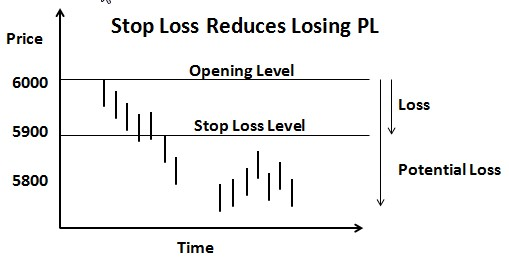
\includegraphics[width=9cm]{chp5b_StopLoss1}
\caption[Situation in which using a stop loss is beneficial]{Situation in which using a stop loss is beneficial, with a losing PL being reduced.}
\label{fig:chp5:sloss1}
\end{figure}

\begin{figure}[tbph]
\centering
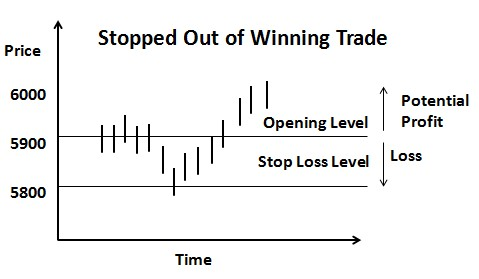
\includegraphics[width=9cm]{chp5b_StopLoss2}
\caption[Situation in which using a stop loss is detrimental]{Situation in which using a stop loss is detrimental, being \textquotedblleft stopped out" of an ultimately winning trade.}
\label{fig:chp5:sloss2}
\end{figure}

Figure \ref{fig:chp5:sloss1} shows the situation in which a stop loss is beneficial. The potential large loss is reduced to the value of the stop loss value. Figure \ref{fig:chp5:sloss2} illustrates the alternative scenario of being \textquotedblleft Stopped Out" of an ultimately winning trade, an undesirable outcome. It is the ratio of these scenarios that ultimately determines whether using a stop loss is a sound strategy.

% latex table generated in R 3.1.0 by xtable 1.7-3 package
% Wed Jul 09 19:03:39 2014
\begin{table}[ht]
\centering
\caption[Results from a system based on SMA with stop loss]{Results from a system based on SMA with stop loss.} 
\label{tab:sma_results_Sloss}
\begin{tabular}{lcccccccc}
  \toprule Mkt & S Loss & LongPL & ShortPL & L Win \% & L Trades & S Win \% & S Trades & SMA \\ 
  \midrule Dax & -50 & 3652 & 6618 & 51 & 2070 & 42 & 1360 & 0 \\ 
  Dax & -100 & 1392 & 5272 & 54 & 2070 & 50 & 1360 & 0 \\ 
  CAC & -50 & -172 & 5178 & 50 & 2012 & 47 & 1475 & 0 \\ 
  CAC & -100 & -1822 & 4658 & 50 & 2012 & 50 & 1475 & 0 \\ 
  FTSE & -50 & 1114 & 6303 & 50 & 2044 & 43 & 1389 & 0 \\ 
  FTSE & -100 & -885 & 1892 & 51 & 2044 & 47 & 1389 & 0 \\ 
  Dow & -50 & -18212 & -8229 & 32 & 2125 & 22 & 1297 & 0 \\ 
  Dow & -100 & -11771 & -14696 & 49 & 2125 & 36 & 1297 & 0 \\ 
  Nikkei & -50 & 8258 & 33882 & 38 & 1643 & 39 & 1696 & 0 \\ 
  Nikkei & -100 & 2550 & 25582 & 47 & 1643 & 48 & 1696 & 0 \\ 
  AORD & -50 & 4008 & 3730 & 54 & 2230 & 49 & 1219 & 0 \\ 
  AORD & -100 & 2881 & 2149 & 54 & 2230 & 50 & 1219 & 0 \\ 
   \bottomrule \end{tabular}
\end{table}


Comparing Tables \ref{tab:sma_results} and \ref{tab:sma_results_Sloss}
it can be seen that applying the stop loss has been on the whole beneficial to the results obtained, with the exception of those from the Dow which were markedly negatively impacted. Essentially losing trades have been truncated while winning trades have been left to develop. One question that needs to be addressed is what value is appropriate for a stop loss. If the value is large the benefits of cutting losses is lost, whereas if it is too small a large number of trades will be \textquotedblleft stopped out". Many traders use a value based on the Average True Range (see Chapter \ref{Chapter3} section \ref{chp3:atr} for details) as this allows for the volatility of a particular market.

\subsection{Moving Average Convergence/Divergence (MACD)}
\label{sec:chp4macd}
Moving Average Convergence/Divergence (MACD) is a trend following indicator, developed by \cite{appel2005technical}, that is formed from the relationship of two moving averages, see Appendix \ref{AppendixB} section \ref{appB:MACD} for more details. The value of MACD itself is the difference between two exponential moving averages (EMA), a \textquotedblleft slower" e.g. 26 day value and a \textquotedblleft faster" e.g. 12 day value. In addition an EMA of the MACD value is calculated, which is set to 9 days in the following algorithm, which acts as a \textquotedblleft signal" line.
 
The MACD is generally used two ways. Firstly, it can be used to derive the general trend of the security so that the market participant can trade with the trend. Secondly, it can be employed to identify periods when the market is \textquotedblleft over-bought" or \textquotedblleft over-sold" and can be expected to reverse direction \citep{MACD2}.

In order to identify the trend of a market using the MACD indicator, the relative values of the MACD itself and the signal line are used. If the value of the MACD exceeds the signal it is considered \textquotedblleft bullish" and the market is expected to rise in price. Similarly in the opposite situation where the value of the signal is greater than the MACD the trend of the market is expected to be down. 

Table \ref{tab:mac_trend_results} lists the results of using the MACD indicator in just such a way. The MACD value itself is generated using the EMA of the opening prices with values of 26 and 12 for the slow and long averages and a value of 9 days for the indicator line. 

The trading algorithm splits the results into two values, days when the system expected the market to rise and days when a market decline were predicted (see Appendix \ref{AppendixA} section \ref{appA:macd_xov} for details of the R code used). At the start of each day if the MACD value exceeds the signal line the algorithm adds the value of the close price minus the opening price to the \textquotedblleft Long PL" running total. Likewise in the opposite situation with the signal line greater than the MACD, the value of the open price minus the close price is added to the \textquotedblleft Short PL". Table \ref{tab:mac_trend_results} lists the results of the algorithm run against a variety of national indices.

% latex table generated in R 3.1.0 by xtable 1.7-3 package
% Mon Aug 11 19:25:42 2014
\begin{table}[ht]
\centering
\caption[Results from a system using MACD as a trend indicator]{Results from a system using MACD as a trend indicator.} 
\label{tab:mac_trend_results}
\begin{tabular}{lcccccc}
  \toprule Mkt & LongPL & ShortPL & L Win \% & Av L PL & S Win \% & Av S PL \\ 
  \midrule DAX & -791 & 1424 & 53 & 0 & 48 & 1 \\ 
  CAC & -4153 & 2188 & 49 & -2 & 49 & 1 \\ 
  FTSE & 63 & -839 & 51 & 0 & 48 & 0 \\ 
  Dow & 5592 & -5190 & 53 & 3 & 46 & -3 \\ 
  Nikkei & -4078 & 14064 & 49 & -2 & 52 & 8 \\ 
  AORD & 2563 & 1569 & 54 & 1 & 49 & 1 \\ 
   \bottomrule \end{tabular}
\end{table}



\subsection{Aroon Indicator}
Developed by Tushar Chande, the Aroon indicator was designed to identify trending markets \citep{chande1994new}. The word aroon means \textquotedblleft dawn's early light" in Sanskrit and this indicator tries to pin point the dawning of a new trend.  Essentially it is a measure of the time since the occurrence of a high/low price in a particular period. Further details can be seen in Appendix \ref{AppendixB} section \ref{appB:aroon}.

% latex table generated in R 3.1.0 by xtable 1.7-3 package
% Mon Aug 11 19:25:43 2014
\begin{table}[ht]
\centering
\caption[Results from a system based on the Aroon indicator]{Results from a system based on the Aroon indicator.} 
\label{tab:aroon_results}
\begin{tabular}{lcccccc}
  \toprule Mkt & LongPL & ShortPL & L Win \% & Av L PL & S Win \% & Av S PL \\ 
  \midrule DAX & 5308 & 5257 & 56 & 3 & 51 & 4 \\ 
  CAC & -1638 & 4919 & 50 & -1 & 52 & 4 \\ 
  FTSE & 3042 & 5715 & 52 & 2 & 51 & 5 \\ 
  Dow & 12131 & 3811 & 55 & 7 & 49 & 3 \\ 
  Nikkei & -4852 & 12013 & 49 & -3 & 52 & 10 \\ 
  AORD & 3735 & 3540 & 55 & 2 & 50 & 3 \\ 
   \bottomrule \end{tabular}
\end{table}


Table \ref{tab:aroon_results} shows the results of applying the Aroon algorithm (shown in Appendix \ref{AppendixA} section \ref{appA:aroon}) on the data of the national indices. The results are promising with the indicator making positive predictions in most of the markets and doing particularly well in declining markets. 

% latex table generated in R 3.1.0 by xtable 1.7-3 package
% Wed Jun 11 06:51:57 2014
\begin{table}[ht]
\centering
\caption[Aroon trend indicator with Stop Loss]{Aroon trend indicator with stop loss.} 
\label{tab:aroon_results_sloss}
\begin{tabular}{lcccccc}
  \toprule Mkt & LongPL & ShortPL & L Win \% & Av L PL & S Win \% & Av S PL \\ 
  \midrule Dax & 5410 & 7465 & 56 & 3 & 50 & 6 \\ 
  CAC & -1224 & 6086 & 50 & -1 & 52 & 5 \\ 
  FTSE & 3091 & 8015 & 52 & 2 & 51 & 7 \\ 
  Dow & -5922 & -9341 & 49 & -3 & 37 & -8 \\ 
  Nikkei & 3153 & 22177 & 46 & 2 & 47 & 18 \\ 
  AORD & 3786 & 4159 & 55 & 2 & 50 & 4 \\ 
   \bottomrule \end{tabular}
\end{table}


The affects of using a stop loss with the Aroon indicator was investigated and the results shown in Table \ref{tab:aroon_results_sloss}. The use of a stop loss was beneficial in all cases except the Dow, in which case it had a catastrophic impact turning a winning system into a losing one.  The impact of the stop loss is shown in Table \ref{tab:aroon_results_sloss_diff} which lists the difference in PL between the original results without a stop loss and the revised ones with it.

% latex table generated in R 3.1.0 by xtable 1.7-3 package
% Fri Jul 11 07:22:26 2014
\begin{table}[ht]
\centering
\caption[Impact of using stop loss with Aroon trend indicator]{Impact of using stop loss with Aroon trend indicator.} 
\label{tab:aroon_results_sloss_diff}
\begin{tabular}{lcc}
  \toprule Market & Long Difference & Short Difference \\ 
  \midrule Dax & 102 & 2208 \\ 
  CAC & 414 & 1167 \\ 
  FTSE & 49 & 2300 \\ 
  Dow & -18053 & -13152 \\ 
  Nikkei & 8005 & 10164 \\ 
  AORD & 51 & 619 \\ 
   \bottomrule \end{tabular}
\end{table}


\section{Market Reversal Indicators}
The alternative to trend detection indicators are market reversal indicators, designed to identify when a trend may be ending and the market will start to move in the opposite direction. Many traders advocate that this type of trading should be avoided and cite the old phrase \textquotedblleft never try to catch a falling knife". Nevertheless a variety of market reversal technical indicators are explored and their effectiveness noted.

\subsection{Parabolic Stop-and-Reverse  (SAR)}
The parabolic stop-and-reverse (SAR) is a method to calculate a trailing stop. This technical indicator was developed by J. Welles Wilder and is detailed in his book New Concepts in Technical Trading Systems \citep{wilder1978new}. A trailing stop is related to the stop loss explored previously but differs in that it is adjusted as the market moves. The level of this of kind of stop loss is amended periodically such that it is a certain amount away from the high or low value of a market. As the the market makes new highs it is adjusted up or down if the market makes new lows. The parabolic SAR calculates the point at which a long trade would be closed and a short position entered, the assumption being that the market participant is always in the market either short or long. More details on the theory and calculations to generate the parabolic SAR can be found in Appendix \ref{AppendixB} section \ref{appB:sar}.  

Table \ref{tab:sar_results} lists the results from passing a variety of national index data sets to an algorithm using the parabolic SAR. The R code used to generate these results can be seen in See Appendix \ref{AppendixA} section \ref{appA:sar}. On the whole the results from these initial tests are very disappointing. Only three of the national indices generated positive results and only the Japanese Nikkei provided reasonable returns.

% latex table generated in R 3.1.0 by xtable 1.7-3 package
% Sun Jun 22 08:27:42 2014
\begin{table}[ht]
\centering
\caption[Results from a system based on the SAR indicator]{Results from a system based on the SAR indicator.} 
\label{tab:sar_results}
\begin{tabular}{lcccccc}
  \toprule Mkt & LongPL & ShortPL & L Win \% & Av L PL & S Win \% & Av S PL \\ 
  \midrule Dax & -3856 & -2353 & 53 & -2 & 48 & -2 \\ 
  CAC & -5584 & 1034 & 49 & -3 & 49 & 1 \\ 
  FTSE & -1141 & -1663 & 51 & -1 & 48 & -1 \\ 
  Dow & -1301 & -11112 & 52 & -1 & 46 & -7 \\ 
  Nikkei & -5767 & 12424 & 49 & -3 & 52 & 8 \\ 
  AORD & 2071 & 1097 & 53 & 1 & 49 & 1 \\ 
   \bottomrule \end{tabular}
\end{table}


\subsection{MACD as reversal Indicator}
MACD can also be used as a reversal indicator. Recalling that the MACD is formed from the relationship of two moving averages, when the faster one moves sharply away from the slower one (i.e.the value of MACD rises) this could be an indication of an \textquotedblleft over-bought" market and that a reversal is approaching. In this situation the trader would place a sell trade. The opposite is true for a large negative MACD, and it is postulated that the market may well reverse upwards. 

Table \ref{tab:mac_ob_results} shows the results of applying the algorithm shown in Appendix \ref{AppendixA} section \ref{appA:macd_ob} on the data of the national indices. In the algorithm the 15\% and 85\% quantile of the MACD value is calculated and this is used to decide on the reversal point. Once the 85\% value is exceeded the algorithm predicts a reversal will occur and trades short, the opposite is true for the 15\% level which triggers a long trade. Overall the results are very modest, with small positive gains being seen in 5 of the 6 national indices. 

% latex table generated in R 3.1.0 by xtable 1.7-3 package
% Sun Aug 31 09:29:26 2014
\begin{table}[ht]
\centering
\caption[Results from a system based on MACD as trend reversal indicator]{Results from a trading system based on MACD being used as a trend reveral indicator.} 
\label{tab:mac_ob_results}
\begin{tabular}{lcccccc}
  \toprule Mkt & LongPL & ShortPL & L Win \% & Av L PL & S Win \% & Av S PL \\ 
  \midrule DAX & 391 & 407 & 49 & 1 & 48 & 1 \\ 
  CAC & -545 & 2657 & 51 & -1 & 55 & 5 \\ 
  FTSE & 2080 & 1649 & 53 & 4 & 53 & 3 \\ 
  Dow & 3882 & -807 & 52 & 7 & 48 & -2 \\ 
  Nikkei & 199 & 2828 & 51 & 0 & 52 & 6 \\ 
  AORD & -319 & -584 & 50 & -1 & 49 & -1 \\ 
   \bottomrule \end{tabular}
\end{table}


\section{Momentum Indicators}
Momentum indicators are closely related to the trend indicators introduced in section \ref{sec:trend}. They are concerned with trending markets but differ in that the strength of the trend is also included in the information the indicator attempts to portray.

\subsection{Stochastic Oscillator}
The stochastic indicator is one of the oldest in widespread use today having been developed by George Lane in the 1950s \citep{lane1986using}. It measures the relative position of a market's closing price in the range between the low and high of the period of interest. This is of interest as some market participants believe that financial markets essentially swing between price boundaries marked by where the market closes in this range \citep{williams2011long}. Thus markets increase until the close is at the top of this range before changing direction and moving down until it is at the bottom of the high low range.

The stochastic is usually represented by two lines \%K which is the position of the price within this high low envelope described above, and \%D a moving average of \%K (see Appendix \ref{AppendixB} section \ref{appB:stoch} for more details). It can be used a number of ways and one popular technique is to go long when the \%K crosses above \%D and to go short in the opposite situation. Table \ref{tab:stoch_results} lists the results from passing a variety of national index data sets to an algorithm which uses the relative position of \%K and \%D to decide which way to trade. The R code used to generate these results can be seen in See Appendix \ref{AppendixA} section \ref{appA:stoch}.

% latex table generated in R 3.1.0 by xtable 1.7-3 package
% Fri Jul 11 07:22:28 2014
\begin{table}[ht]
\centering
\caption[Results from a system based on the Stochastic indicator]{Results from a system based on the Stochastic indicator.} 
\label{tab:stoch_results}
\begin{tabular}{lcccccc}
  \toprule Mkt & LongPL & ShortPL & L Win \% & Av L PL & S Win \% & Av S PL \\ 
  \midrule Dax & -28 & 1673 & 53 & 0 & 49 & 1 \\ 
  CAC & -4540 & 1817 & 48 & -3 & 48 & 1 \\ 
  FTSE & -73 & -744 & 51 & 0 & 48 & 0 \\ 
  Dow & 867 & -9414 & 53 & 0 & 46 & -5 \\ 
  Nikkei & -10591 & 7802 & 48 & -6 & 51 & 5 \\ 
  AORD & 2839 & 1780 & 54 & 2 & 49 & 1 \\ 
   \bottomrule \end{tabular}
\end{table}


The results from Table \ref{tab:stoch_results} for this system are very modest with only the Australian ORD showing positive values for both long and short trades. Adding a stop loss of 100 points increases the PL across the board except for the case of the Dow where again the stop loss has had a detrimental affect. The results from using a stochastic based system with a stop loss can be seen in Table \ref{tab:stoch_results_sloss}.

% latex table generated in R 3.1.0 by xtable 1.7-3 package
% Sun Aug 31 09:29:28 2014
\begin{table}[ht]
\centering
\caption[Results from a system based on the Stochastic indicator with a stop loss]{Results from a system based on the Stochastic indicator with a stop loss.} 
\label{tab:stoch_results_sloss}
\begin{tabular}{lcccccc}
  \toprule Mkt & LongPL & ShortPL & L Win \% & Av L PL & S Win \% & Av S PL \\ 
  \midrule DAX & 1173 & 3889 & 52 & 1 & 48 & 2 \\ 
  CAC & -3493 & 2730 & 48 & -2 & 48 & 2 \\ 
  FTSE & 1640 & 1424 & 51 & 1 & 48 & 1 \\ 
  Dow & -13969 & -27388 & 45 & -8 & 37 & -16 \\ 
  Nikkei & 1647 & 17977 & 45 & 1 & 46 & 10 \\ 
  AORD & 3028 & 1974 & 54 & 2 & 49 & 1 \\ 
   \bottomrule \end{tabular}
\end{table}

 
\subsection{Rate of Change (ROC)}
The Rate of Change (ROC) indicator is a simple and widely observed technical indicator. It is the difference between the current price and the price several observations ago. See Appendix \ref{AppendixB} section \ref{appB:roc} for details. If this value is large, either positive or negative it is indicative of a strongly trending market with a lot of momentum either upwards or downwards. The R code for a trading system exploiting these ideas can be seen in Appendix \ref{AppendixA} section \ref{appA:roc}. The results can be seen in Table \ref{tab:mac_roc_results} which lists the results from passing a variety of national index data sets to the algorithm.

% latex table generated in R 3.1.0 by xtable 1.7-3 package
% Thu May 29 17:56:17 2014
\begin{table}[ht]
\centering
\caption[Naive Long System - Close to Close]{Naive Long System changed such that the trading period is the previous close price minus today's close.} 
\label{tab:mac_roc_results}
\begin{tabular}{lcccccc}
  \toprule Mkt & LongPL & ShortPL & L Win \% & L Trades & S Win \% & S Trades \\ 
  \midrule Dax & 930 & 148 & 50 & 529 & 50 & 529 \\ 
  CAC & 952 & 956 & 53 & 538 & 51 & 538 \\ 
  F100 & 1147 & 1880 & 51 & 530 & 51 & 530 \\ 
  Dow & 8517 & 3396 & 58 & 528 & 49 & 528 \\ 
  Nik & 2971 & 2546 & 50 & 516 & 52 & 516 \\ 
  Oz & 271 & 1325 & 51 & 532 & 52 & 532 \\ 
   \bottomrule \end{tabular}
\end{table}


%If previous ROC was greater or smaller than 0:
%% latex table generated in R 3.1.0 by xtable 1.7-3 package
% Fri May 30 19:26:08 2014
\begin{table}[ht]
\centering
\caption[Naive Long System - Close to Close]{Naive Long System changed such that the trading period is the previous close price minus today's close.} 
\label{tab:mac_roc2_results}
\begin{tabular}{lcccccc}
  \toprule Mkt & LongPL & ShortPL & L Win \% & L Trades & S Win \% & S Trades \\ 
  \midrule Dax & -1118 & 1189 & 52 & 1836 & 48 & 1658 \\ 
  CAC & -5648 & 715 & 48 & 1815 & 48 & 1767 \\ 
  F100 & -4197 & -4495 & 50 & 1813 & 47 & 1713 \\ 
  Dow & -4826 & -15003 & 51 & 1848 & 44 & 1669 \\ 
  Nik & -17576 & 125 & 47 & 1739 & 50 & 1694 \\ 
  Oz & -429 & -1508 & 52 & 1872 & 47 & 1657 \\ 
   \bottomrule \end{tabular}
\end{table}


\section{Break-out systems}
\label{sec:bout}
This section explores some trading systems that use a particular price as the indicator to place a trade. The first system uses the simple idea of trading when the previous day's high or low is passed. The second idea is related to the results generated in Chapter \ref{Chapter3}, where the 90\% quantile for the day's minor move was calculated. The system tested here is to simply trade long or short when this point is reached in a day.

%----------------------------------------------------------------
% ---------------------------  Break Out ------------------------
\subsection{Daily High/Low Breakout System}
\label{sec:chp5:bout_sys}
Table \ref{tab:hl_bout_sys} lists the results from a trading system based around the idea of trading after the previous day's high or low price has been breached. The R code used to generate these results can be seen in See Appendix \ref{AppendixA} section \ref{appA:bout_sys}.

% latex table generated in R 3.1.0 by xtable 1.7-3 package
% Tue Aug 12 20:06:52 2014
\begin{table}[ht]
\centering
\caption[Results from the Daily High/Low Breakout System]{Results from the Daily High/Low Breakout System.} 
\label{tab:hl_bout_sys}
\begin{tabular}{lcccccc}
  \toprule Mkt & LongPL & ShortPL & L Win \% & Av L PL & S Win \% & Av S PL \\ 
  \midrule DAX & 12225 & 13411 & 55 & 7 & 54 & 8 \\ 
  CAC & 3491 & 6955 & 53 & 2 & 53 & 4 \\ 
  FTSE & 13189 & 18481 & 59 & 7 & 59 & 12 \\ 
  Dow & -19598 & -28337 & 42 & -11 & 38 & -17 \\ 
  Nikkei & 31988 & 43554 & 57 & 19 & 58 & 27 \\ 
  AORD & 17225 & 19184 & 66 & 10 & 65 & 13 \\ 
   \bottomrule \end{tabular}
\end{table}


Referring to Table \ref{tab:hl_bout_sys} we can see that this system produces good results, with the exception of the US Dow. This ties in with the data in Chapter \ref{Chapter3} Table \ref{tab:closeHL} which shows that the Dow only closes outside of the previous low or high price a relatively low number of times. Likewise good results are seen with the Japanese Nikkei from the breakout system and this tallies with the high proportion of the time in which it closes above or below the previous day's high or low.

%----------------------------------------------------------------
% ---------------------------  90% Quant ------------------------
\subsection{Break Out of 90\% Quantile Level}
A second system utilising the break-out concept is presented in this section. In Chapter \ref{Chapter3} one characteristic of the markets was noted, namely that each day the market moves from its opening price to a low price and then to a high price (not necessarily in any particular order). One of these moves (O-H vs O-L) is greater than the other was termed the major move and the smaller move was called the minor move. The algorithm generating the results in this section (see Appendix \ref{AppendixA} section \ref{appA:bout_Quant90}) makes a long or short trade after the market has passed the 90\% quantile of the minor move. Table \ref{tab:q_90_results} lists the results from this algorithm.

% latex table generated in R 3.0.2 by xtable 1.7-1 package
% Fri May 16 23:05:30 2014
\begin{table}[ht]
\centering
\caption[Base System 3]{Base System 3 - 90 Quantile.} 
\label{tab:q_90_results}
\begin{tabular}{lcccccc}
  \toprule Mkt & LongPL & ShortPL & L Win \% & L Trades & S Win \% & S Trades \\ 
  \midrule Dax & 7841 & 6371 & 56 & 1382 & 53 & 1501 \\ 
  CAC & 2647 & 5085 & 54 & 1408 & 52 & 1566 \\ 
  F100 & 10758 & 15295 & 56 & 1627 & 54 & 1561 \\ 
  Dow & -30262 & -34854 & 39 & 1238 & 37 & 1265 \\ 
  Nik & 23606 & 31830 & 58 & 1438 & 56 & 1554 \\ 
  Oz & 16730 & 19357 & 63 & 1805 & 62 & 1647 \\ 
   \bottomrule \end{tabular}
\end{table}


\section{Candlestick Patterns}
As previously noted in Chapter \ref{Chapter2} section \ref{sec:candlesticks} candlestick patterns are visual representations of price movements over the course of a particular time period (often a day) in terms of the market's opening, closing, high and low prices. The pattern generated from these price markets are categorised and named depending upon the visual shape they produce. Thus candlestick patterns represent the counter forces of buyers and sellers throughout the trading period. This section analyses some well known candlestick patterns for predictive power in making trading decisions \citep{Lu201465}.

% -----------------  Hammer -------------------
\subsection{Hanging Man, Hammer, Inverted Hanging Man and Shooting Star}
Four well-known patterns that are generally considered to indicate the possible end of a trend and the start of a reversal are the so-called Hanging Man, Hammer, Inverted Hanging Man and Shooting Star candlestick patterns. 

\begin{figure}[tbph]
\centering
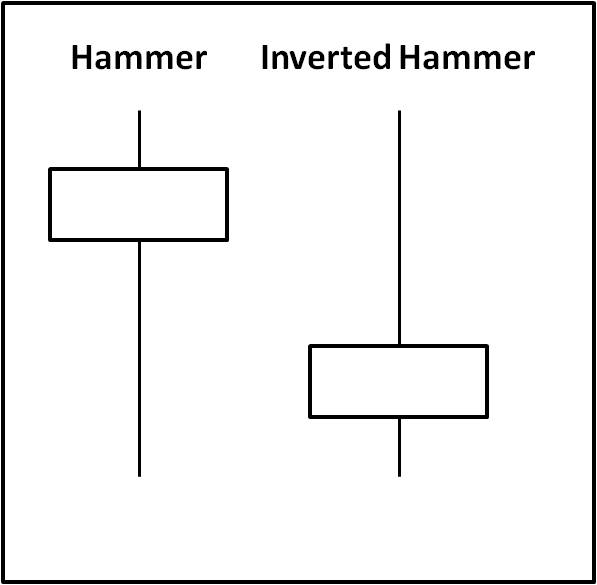
\includegraphics[width=5cm]{chp5e_candle_hammer}
\caption[Hammer and Inverted Hammer candlestick patterns]{Hammer and Inverted Hammer candlestick patterns.}
\label{fig:chp5e:hammer}
\end{figure}

Figure \ref{fig:chp5e:hammer} is a diagram of a Hammer and Inverted Hammer patterns. Both patterns have a small \textquotedblleft body" (the distance between the open and close prices) and a long \textquotedblleft shadow" (the distance between the high and low prices). In the diagrams presented here a white candlestick means the market price increased over the course of the day while a black one means the market fell. The body of the candlestick is white in this case, indicating that the market moved up (the closing price was above the opening price), although by only a small amount. Hammer and Inverted Hammer differ in that the long shadow in hammer is generated from a low price whereas the shadow of Inverted Hammer goes upwards as it is indicative of the period's high price.

\begin{figure}[tbph]
\centering
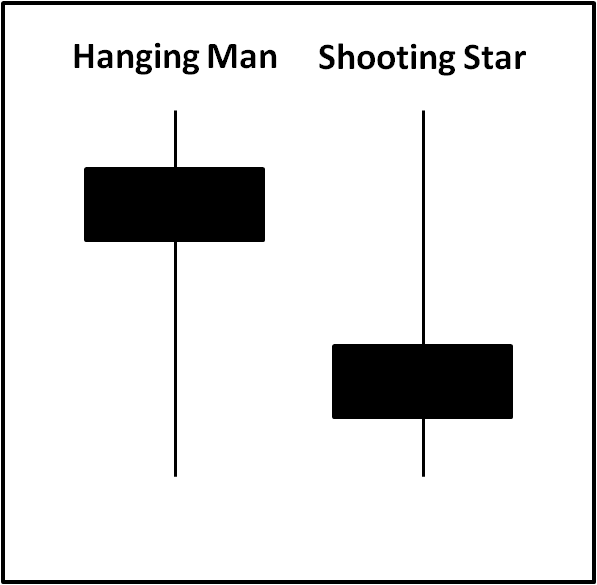
\includegraphics[width=5cm]{chp5e_candle_shoot_star}
\caption[Hanging Man and Shooting Star candlestick patterns]{Hanging Man and Shooting Star candlestick patterns.}
\label{fig:chp5e:shoot_star}
\end{figure}

Figure \ref{fig:chp5e:shoot_star} is a diagram of Hanging Man and Shooting Star, these being the opposite to Hammer and Inverted Hammer. In this case the market direction is down, albeit only by a small amount, and thus the body of the candlestick is a different colour, in this case black. Again both patterns have long shadows, the direction of which determines if the pattern is Hanging Man or Shooting Star.

\begin{figure}[tbph]
\centering
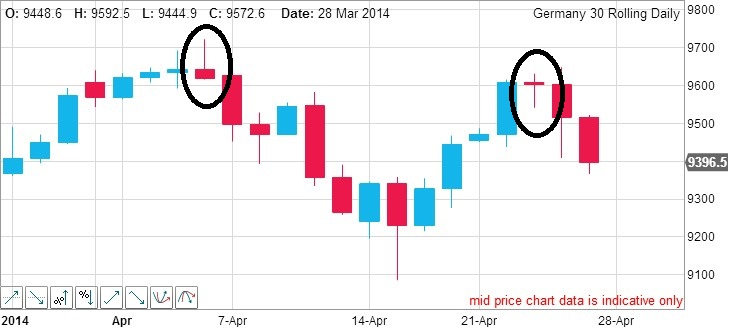
\includegraphics[width=12cm]{chp5e_candle_shoot_star_apr_dax_jp}
\caption [DAX candlestick patterns occurring in April 2014.]{Daily candlestick patterns from the German DAX over 22 days in April 2014 with Shooting Star and Hanging Man circled.}
\label{fig:chp5e:shoot_star_dax}
\end{figure}

Both sets of patterns Hammer/Inverted Hammer and Hanging Man/Shooting Star are considered to indicate that a trend is coming to a close and a reversal could be looming. In the case of Hammer/Inverted Hammer if they are encountered during a down trend they could indicate that the selling pressure is easing and a market move to the upside could happen soon. The opposite is true for Hanging Man/Shooting Star. When these are encountered in an up trend they often indicate that the trend is ending and a reversal may occur. Figure \ref{fig:chp5e:shoot_star_dax} shows daily candlestick patterns for the German DAX over 22 days in April 2014. A Shooting Star is circled on the 6th April and a Hanging Man on the 23rd April. In each case they occur while the market is rising and in each case it reverses immediately afterwards.

In order to have a system based on candlestick patterns, the pattern itself must be identified in code. A Hammer and Hanging Man are essentially the same pattern except Hammer has a close higher than the open whereas Hanging Man represents a decline in the price. For these patterns three components are defined, the length of the upper shadow (short), the size of the body (short) and the length of the lower shadow. In the trading system that follows these were defined as:

\begin{enumerate}
\item Upper Shadow - the value of the day's high minus the high of the body is less than 10\% the total High-Low range.
\item Body - is larger than 10\% the total High-Low range.
\item Lower Shadow - the value of the day's low minus the low of the body is greater than 66\% of the High-Low range.
\end{enumerate}

Analysing the DAX data set running from 2000 to 2013 with 3570 observations, and using the criteria described above 35 Hammer and 48 Hanging Man patterns can be detected. 

Inverted Hammer and Shooting Star are again the same pattern except in Inverted Hammer the price rose. In the later system these are defined as:

\begin{enumerate}
\item Upper Shadow - the value of the day's high minus the high of the body is at least 66\% the total High-Low range.
\item Body - is larger than 10\% the total High-Low range.
\item Lower Shadow - the value of the day's low minus the low of the body is less than 10\% of the High-Low range.
\end{enumerate}

Considering the DAX data set again, occurrences of these patterns are quite rare with 30 Inverted Hammers and 17 Shooting Stars in 3570 observations.

Results from a trading system based on the Hammer/Inverted Hammer can be seen in Table \ref{tab:hammer_results} and the R code in Appendix \ref{AppendixA} section \ref{appA:Hammer}. The algorithm simply places a buy the day after a Hammer or Inverted Hammer occur, the assumption being that these patterns indicate that the market is about to rise.


% latex table generated in R 3.1.0 by xtable 1.7-3 package
% Sat Jun 07 07:56:31 2014
\begin{table}[ht]
\centering
\caption[Hammer System]{Results from Hammer / Inverted Hammer.} 
\label{tab:hammer_results}
\begin{tabular}{lcccc}
  \toprule Mkt & LongPL & L Win \% & L Trades & Av L PL \\ 
  \midrule Dax & 594 & 53 & 126 & 5 \\ 
  CAC & -793 & 44 & 149 & -5 \\ 
  FTSE & 834 & 58 & 188 & 4 \\ 
  Dow & 2097 & 59 & 88 & 24 \\ 
  Nikkei & -2202 & 48 & 147 & -15 \\ 
  AORD & -809 & 46 & 236 & -3 \\ 
   \bottomrule \end{tabular}
\end{table}


An alternative approach is to look for Hammer and Inverted Hammer patterns occurring in a down trend, in which case it could signal the end of the down trend and the start of a reversal. Table \ref{tab:hammer_aroon_results} shows the results of using the Hammer and Inverted Hammer to predict a price rise during a down trend. An aroon down value of greater than 65 (with a 20 day look back period) is used to define the down trend. The algorithm can be seen in Appendix \ref{AppendixA} section \ref{appA:Hammer_aroon}.  


% latex table generated in R 3.1.0 by xtable 1.7-3 package
% Mon Jun 23 18:28:43 2014
\begin{table}[ht]
\centering
\caption[Results from a system based on the Hammer and Inverted Hammer candlestick patterns occurring in a downtrend]{Results from a system based on the Hammer and Inverted Hammer candlestick patterns occurring in a downtrend as defined by the aroon value.} 
\label{tab:hammer_aroon_results}
\begin{tabular}{lcccc}
  \toprule Mkt & LongPL & L Win \% & L Trades & Av L PL \\ 
  \midrule Dax & -187 & 42 & 36 & -5 \\ 
  CAC & -515 & 44 & 55 & -9 \\ 
  FTSE & 281 & 55 & 65 & 4 \\ 
  Dow & 730 & 55 & 22 & 33 \\ 
  Nikkei & -934 & 48 & 58 & -16 \\ 
  AORD & -614 & 41 & 77 & -8 \\ 
   \bottomrule \end{tabular}
\end{table}


%-------------------------------------------------------------
% -----------------  Engulfing Candlestick -------------------
\subsection{Engulfing Candlestick}
\label{sec:eng_cand}
The \textquotedblleft Engulfing" pattern, either Bull or Bear is another widely considered candlestick pattern and is depicted in Figure \ref{fig:chp5e:engulf}. This pattern has a lower low and a higher high than the preceding candlestick and is usually interpreted as indicating a change in direction of the trend. Engulfing candlesticks can be either bullish, where the closing price is above the opening price or bearish when the market moves down.

\begin{figure}[tbph]
\centering
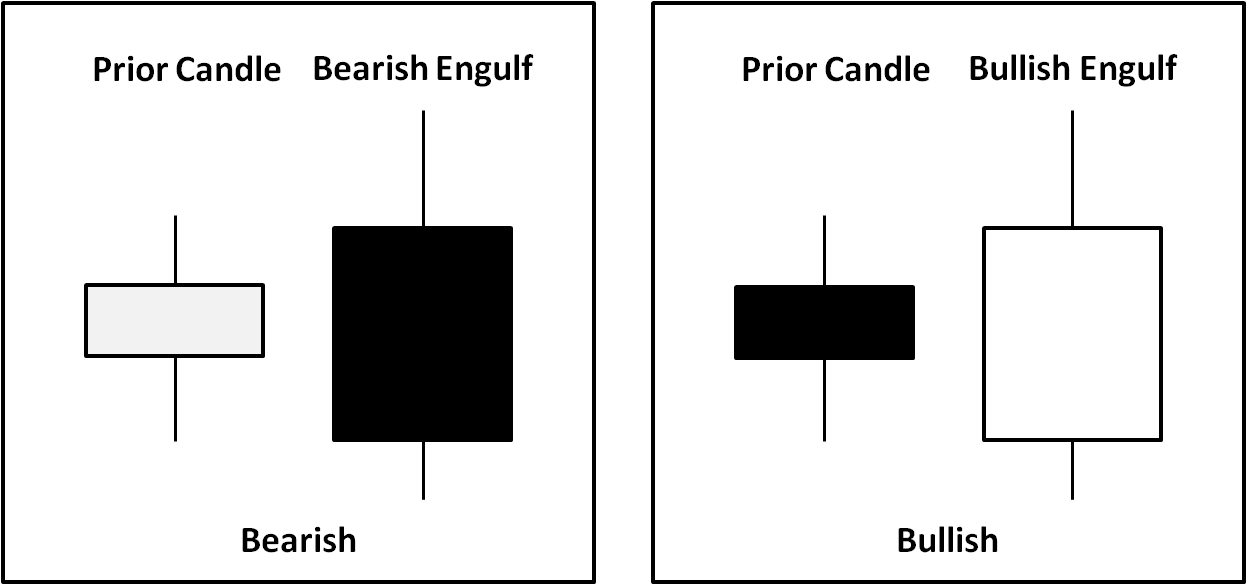
\includegraphics[width=10cm]{chp5e_candle_engulf}
\caption[Engulfing candlestick patterns]{Engulfing candlestick patterns.}
\label{fig:chp5e:engulf}
\end{figure}

Table \ref{tab:engulf_results} lists the results from passing a variety of national index data sets (see Appendix \ref{AppendixA} section \ref{appA:Engulf} for details) to an algorithm that buys or sells the market depending on the presence of an Engulfing pattern.


% latex table generated in R 3.1.0 by xtable 1.7-3 package
% Sun Aug 31 09:29:32 2014
\begin{table}[ht]
\centering
\caption[Results from a system based on the Engulfing candlestick pattern]{Results from a system based on the Engulfing candlestick pattern.} 
\label{tab:engulf_results}
\begin{tabular}{lcccccc}
  \toprule Mkt & LongPL & ShortPL & L Win \% & Av L PL & S Win \% & Av S PL \\ 
  \midrule DAX & -920 & -258 & 44 & -7 & 46 & -2 \\ 
  CAC & -319 & 228 & 45 & -2 & 50 & 1 \\ 
  FTSE & -1721 & 1185 & 51 & -4 & 50 & 3 \\ 
  Dow & -770 & -3662 & 48 & -4 & 35 & -28 \\ 
  Nikkei & -3823 & -1166 & 37 & -39 & 44 & -11 \\ 
  AORD & -6 & -600 & 53 & 0 & 46 & -3 \\ 
   \bottomrule \end{tabular}
\end{table}


Table \ref{tab:engulf_aroon_results} lists the results from extending the algorithm such that trades are only taken in either up or down trends, as defined by the aroon indicator. The R code for the amended algorithm can be see Appendix \ref{AppendixA} section \ref{appA:Engulf_aroon}.

% latex table generated in R 3.1.0 by xtable 1.7-3 package
% Sun Aug 31 09:29:33 2014
\begin{table}[ht]
\centering
\caption[Results from a system based on the Engulfing candlestick pattern in a trending market]{Results from a system based on the Engulfing candlestick pattern in a trending market.} 
\label{tab:engulf_aroon_results}
\begin{tabular}{lcccccc}
  \toprule Mkt & LongPL & ShortPL & L Win \% & Av L PL & S Win \% & Av S PL \\ 
  \midrule DAX & -874 & -513 & 38 & -20 & 43 & -7 \\ 
  CAC & -118 & -666 & 49 & -3 & 30 & -11 \\ 
  FTSE & -1217 & -782 & 47 & -8 & 48 & -3 \\ 
  Dow & 202 & -1154 & 45 & 4 & 44 & -11 \\ 
  Nikkei & -1522 & -1733 & 38 & -59 & 37 & -32 \\ 
  AORD & -49 & -27 & 53 & -1 & 50 & 0 \\ 
   \bottomrule \end{tabular}
\end{table}


%----------------------------------------------------------
% ---------------------------  Doji ------------------------
\subsection{Doji}
Doji is a well-known candlestick pattern that can appear on its own or as a component of a pattern. A Doji forms when the open and close price are similar and there is an upper and lower shadow, thus they often resemble a cross. Variations within Doji include the Dragonfly and Gravestone Doji, see Figure \ref{fig:chp5e:doji}. In an up trend Doji (especially Gravestone) can indicate a reversal could occur and likewise in a down trend a Dragonfly could suggest an upward move is about to start.

\begin{figure}[tbph]
\centering
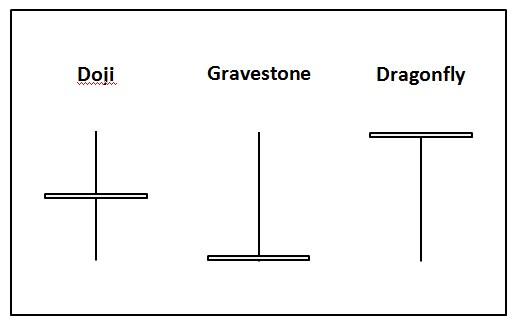
\includegraphics[width=10cm]{chp5e_candle_doji}
\caption[Doji candlestick patterns]{Doji candlestick patterns.}
\label{fig:chp5e:doji}
\end{figure}

Table \ref{tab:doji_aroon_results} lists the results from passing a variety of national index data sets (see Appendix \ref{AppendixA} section \ref{appA:Doji_aroon} for details) to an algorithm that buys or sells the market depending on the presence of a Doji. In an up trend, as identified by the aroon indicator, a Doji or Gravestone is used to initiate a sell and conversely in down trend a Doji or Dragonfly is used as a signal to buy.

% latex table generated in R 3.1.0 by xtable 1.7-3 package
% Thu Jul 10 21:16:47 2014
\begin{table}[ht]
\centering
\caption[Results from a system based on the Doji candlestick pattern in a trending market]{Results from a system based on the Doji candlestick pattern in a trending market.} 
\label{tab:doji_aroon_results}
\begin{tabular}{lcccccc}
  \toprule Mkt & LongPL & ShortPL & L Win \% & Av L PL & S Win \% & Av S PL \\ 
  \midrule Dax & -826 & -1132 & 53 & -8 & 52 & -6 \\ 
  CAC & -747 & -326 & 46 & -6 & 49 & -2 \\ 
  FTSE & -697 & 418 & 53 & -8 & 52 & 3 \\ 
  Dow & -763 & -2869 & 51 & -5 & 50 & -10 \\ 
  Nikkei & 1296 & -2944 & 55 & 12 & 45 & -22 \\ 
  AORD & -115 & 195 & 54 & -1 & 54 & 2 \\ 
   \bottomrule \end{tabular}
\end{table}

 
